\begin{frame}{The Tool for Optimization}
    \framesubtitle{How do we find the minimum?}
    \begin{itemize}
        \item We have defined our goal: find the set of weights $W$ that minimizes the cost function $E(W)$.
        \item The cost function for a neural network is a complex function in a very high-dimensional space (one dimension for each parameter).
        \item We cannot solve for the minimum analytically. Instead, we must search for it using an \bhighlight{iterative optimization algorithm}.
    \end{itemize}
\end{frame}

\begin{frame}{The Tool: Gradient Descent}
    \framesubtitle{The Core Idea}
    \small
    \begin{itemize}
        \item The most common optimization algorithm is \bhighlight{gradient descent}.
        \item The core idea is to start with an initial random guess for the weights ($w^0$) and take small, iterative steps in the direction of the \bhighlight{negative gradient} of the error surface.
        \item \textbf{Analogy:} Imagine a blindfolded hiker trying to find the bottom of a valley. At any point, they feel the slope of the ground under their feet and take a step in the steepest downhill direction. They repeat this process until they reach a point where the ground is flat.
    \end{itemize}
    \begin{figure}
        \centering
        % Source: Optimization II.pdf, Page: 2
        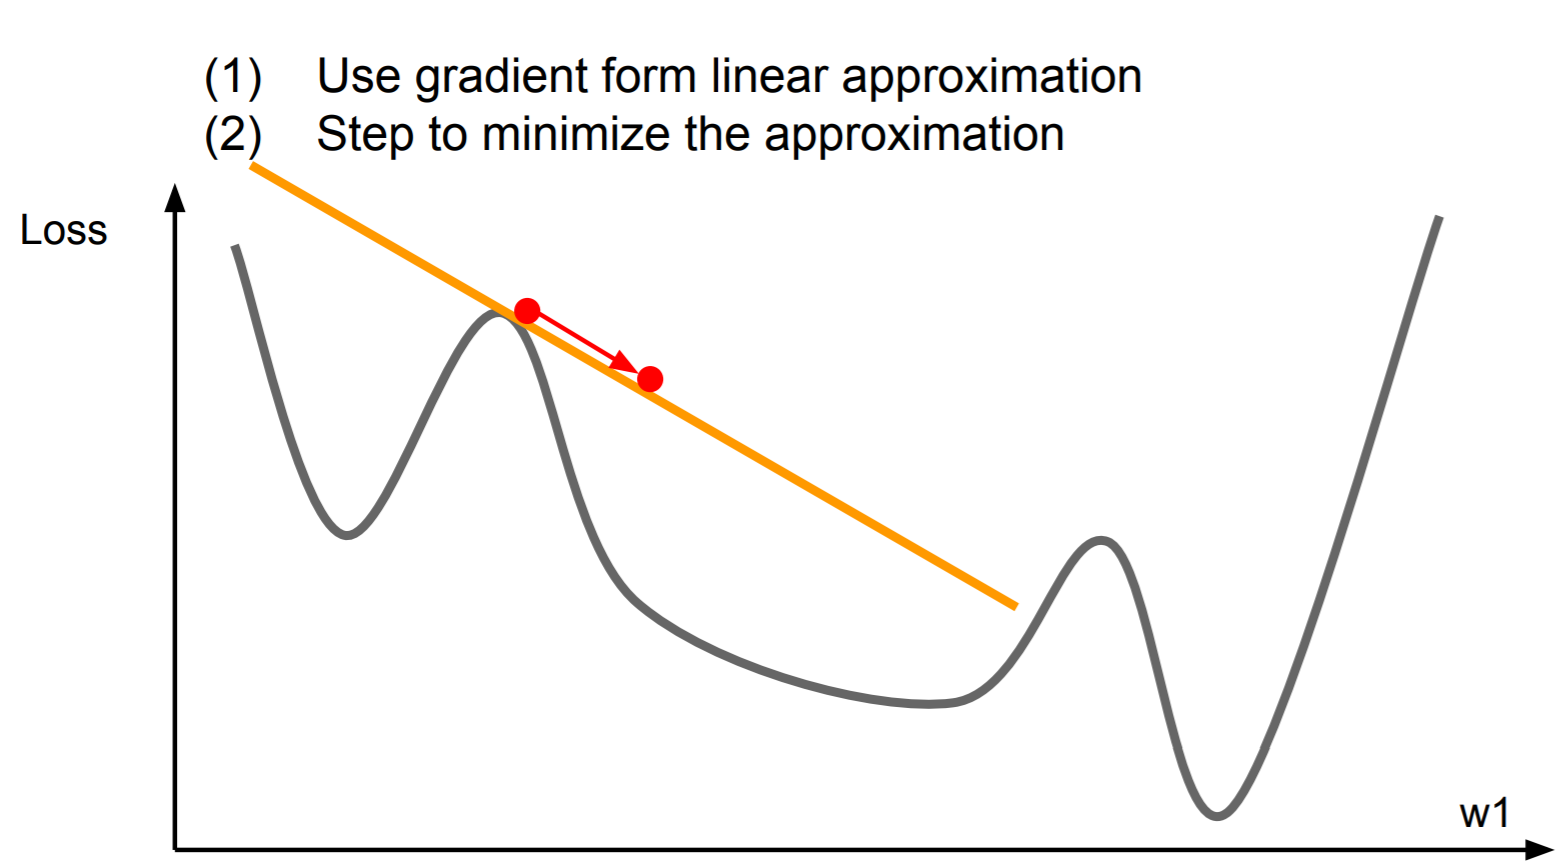
\includegraphics[width=0.4\linewidth]{images/gradient_descent_step.png}
        \caption{A single step of gradient descent. We form a linear approximation of the loss and step to minimize it.}
    \end{figure}
\end{frame}

\begin{frame}{The Tool: Gradient Descent}
    \framesubtitle{What is the Gradient?}
    \begin{itemize}
        \item In a multi-dimensional space, the derivative is called the \bhighlight{gradient}, denoted as $\nabla_{w}J(w)$.
        \item The gradient is a \bhighlight{vector} that contains the partial derivative of the cost function with respect to every single weight in the network:
        \[
            \nabla_{w}J(w) = \left[ \frac{\partial J(w)}{\partial w_0}, \frac{\partial J(w)}{\partial w_1}, \dots, \frac{\partial J(w)}{\partial w_d} \right]^T
        \]
        \item Crucially, the gradient vector always points in the direction of the \bhighlight{steepest ascent} of the cost function. Therefore, the negative gradient points in the direction of the \bhighlight{steepest descent}.
    \end{itemize}
\end{frame}

\begin{frame}{The Tool: Gradient Descent}
    \framesubtitle{The Update Rule}
    \begin{itemize}
        \item At each iteration $t$, we update the entire vector of weights according to the following rule:
        \[
            w^{t+1} = w^{t} - \eta \nabla_{w}J(w^{t})
        \]
        \item Where:
        \begin{itemize}
            \item $w^{t}$ is the vector of all weights in the network at iteration $t$.
            \item $\eta$ (eta) is the \bhighlight{learning rate}, a critical hyperparameter that controls the step size. If it's too small, learning is slow; if it's too large, the algorithm might overshoot the minimum and diverge.
            \item $\nabla_{w}J(w^{t})$ is the \bhighlight{gradient} of the cost function, evaluated at the current weights $w^t$.
        \end{itemize}
    \end{itemize}
\end{frame}

\begin{frame}{The Tool: Gradient Descent}
    \framesubtitle{The Challenge: Computing the Gradient}
    \begin{itemize}
        \item The update rule is simple, but how do we compute the gradient $\nabla_{w}J$ for a deep network with potentially millions of parameters?
        \item The cost function is a deeply nested composite function:
        \[ E(W) = \text{loss}(f(W^{[L]} \dots f(W^{[2]}f(W^{[1]}x))\dots)) \]
        \item Calculating the derivative for each weight by hand is impossible and computationally inefficient. We need an automated and efficient method.
    \end{itemize}
\end{frame} 

\begin{frame}{The Tool: Gradient Descent}
    \framesubtitle{The Solution: Backpropagation}
    \begin{itemize}
        \item The gradient $\nabla_{w}J$ is computed efficiently using the \bhighlight{backpropagation} algorithm.
        \item Backpropagation is \bhighlight{not} the training algorithm itself; it is the procedure for efficiently calculating the gradient. Gradient descent is the training algorithm that \emph{uses} this gradient.
        \item It is a clever implementation of the \bhighlight{chain rule} from calculus, combined with \bhighlight{dynamic programming} to avoid re-computing intermediate values.
    \end{itemize}
\end{frame}

\begin{frame}{The Tool: Gradient Descent}
    \framesubtitle{The Two-Step Process of Backpropagation}
    The algorithm works in two stages for each training example (or mini-batch):
    \begin{enumerate}
        \item \textbf{Forward Pass:}
        \begin{itemize}
            \item The input data $x$ is fed into the network.
            \item The computation flows forward through the layers, calculating the pre-activations ($z$) and activations ($a$) at each layer, until the final output $f(x;W)$ is produced.
            \item The loss between the output and the true label $y$ is calculated.
        \end{itemize}
        \item \textbf{Backward Pass:}
        \begin{itemize}
            \item The gradient of the loss is propagated backward from the output layer to the input layer.
            \item At each layer, the algorithm calculates the gradient of the loss with respect to that layer's weights and biases.
        \end{itemize}
    \end{enumerate}
\end{frame}